面向对象编程(OOP)为我们提供了一种思考方式,可以用类及关系来描述现实世界。函数式编程是另一种完全不同的编程范式,它允许我们专注于函数结构,而不是代码的物理结构。学习和使用函数式编程很有用。首先,它是一种新的范式,可使你以非常不同的方式思考。解决问题需要灵活的思维,执着于单一范式的人往往会为任何问题提供类似的解决方案,而最优雅的解决方案需要更好的方法。掌握函数式编程为开发人员提供了一种新技能,可以帮助他们提供更好的问题解决方案。其次,使用函数式编程减少了软件中的错误数量。函数式编程采用独特方法的最大原因之一是:将程序分解为函数,每个函数都不修改数据的状态。\par
本章中,我们将讨论函数式编程的基本模块以及范围。C++20中引入的range为我们提供了一种组合算法的方法,这样就可以处理数据集合。组合算法以便我们可以将它们按顺序应用到数据集合中,这是函数式编程的核心。 \par
本章中,我们将了解以下内容: \par

\begin{itemize}
	\item 函数式编程简介
	\item range库的介绍
	\item 纯函数
	\item 高阶函数
	\item 深入地研究递归
	\item C++中(函数式)的元编程
\end{itemize}

\noindent\textbf{}\ \par
\textbf{编译器要求} \ \par
g++编译器需要添加编译选项 \texttt{-std=c++2a} 来编译本章的代码。可以从这里获取本章的源码文件:https:/​/github.​com/PacktPublishing/Expert-CPP \par

\noindent\textbf{}\ \par
\textbf{函数式编程} \ \par
正如我们前面提到的,函数式编程是一种编程范式。构建程序时,可以将范式视为一种思考方式。C++是一种多范式语言,可以使用它在过程范式中开发程序,即一个接一个地执行语句。第3章中,我们讨论了面向对象方法,涉及到将一个复杂的系统分解为相互通信的对象。另一方面,函数式编程鼓励我们将系统分解为函数,而不是对象。表达式受一些输入,并一个产生输出,输出这可以用作另一个函数的输入。乍一看,似乎很简单,但是函数式编程包含了一些最初感觉很难掌握的规则。然而,当你做到这一点时,大脑就会开启一种新的思维方式——功能性思维方式。 \par 
为了更清楚地说明这一点,我们从一个示例开始演示函数式编程的原理。假设得到了一个整数列表,需要计算其中的偶数个数。唯一的问题是我们应该分别计算所有向量中的偶数,并生成一个新向量,其中包含每个输入向量的计算结果。 \par
输入是一个矩阵,即向量中的向量。在C++中,最简单的表达方式是使用以下类型: \par

\begin{lstlisting}[caption={}]
std::vector<std::vector<int>>
\end{lstlisting}

我们可以通过使用类型别名来进一步简化前面的代码,如下所示: \par

\begin{lstlisting}[caption={}]
using IntMatrix = std::vector<std::vector<int>>;
\end{lstlisting}

下面是对这个问题的说明。我们有一串包含整数的向量,因此得到一个包含偶数计数的vector: \par

\begin{center}
	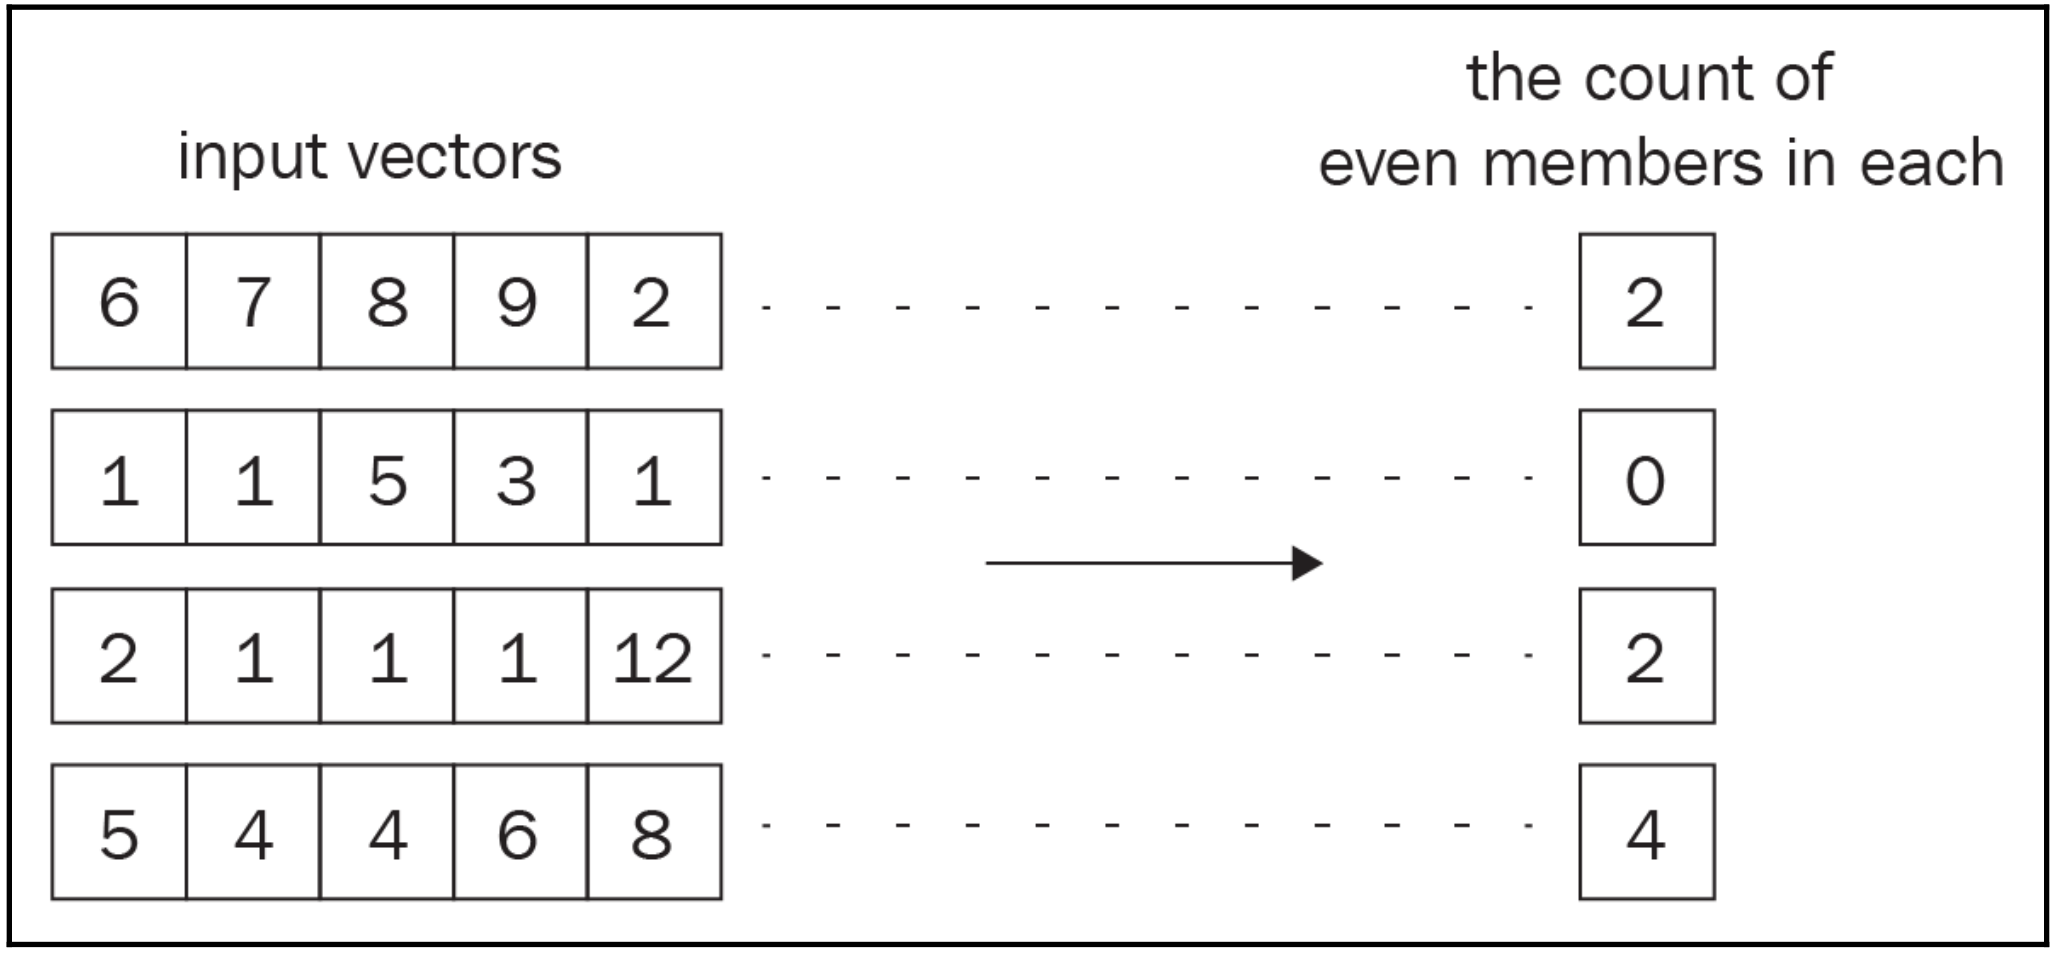
\includegraphics[width=0.6\textwidth]{content/Section-2/Chapter-7/1}
\end{center}

看看下面的函数。它以一个由整数向量组成的vector(也称为矩阵)作为它的参数。该函数计算偶数的数目: \par

\begin{lstlisting}[caption={}]
std::vector<int> count_all_evens(const IntMatrix& numbers)
{
	std::vector<int> even_numbers_count;
	for (const auto& number_line: numbers) {
		int even{0};
		for (const auto& number: number_line) {
			if (number % 2 == 0) {
				++even;
			}
		}
		even_numbers_count.push_back(even);
	}
	return even_numbers_count;
}
\end{lstlisting}

前面的函数保留一个vector来存储每个向量的偶数计数,输入为二维vector。对于检索到的每个vector,都将对其进行循环,并在每次遇到vector中的偶数时在计数器上增加1。完成每个向量的循环后,最终结果推入包含数字列表的vector中。我们现在继续,并将其分解为更小的函数。首先,我们将负责计算偶数的代码部分移动到单独的函数中。 \par
我们把它命名为count\underline{ }evens,如下所示: \par

\begin{lstlisting}[caption={}]
int count_evens(const std::vector<int>& number_line) {
	return std::count_if(number_line.begin(),
	number_line.end(), [](int num){return num % 2 == 0;});
}
\end{lstlisting}

注意如何使用count\underline{ }if()算法。它接受两个迭代器,并将它们分别放在容器的开头和结尾。它还接受第三个参数,一元谓词,集合的每个元素都会调用该谓词。我们传递一个lambda作为一元谓词,也可以使用任何其他可调用实体,例如函数指针、std::function等。 \par
现在有了独立的计数函数,我们可以在count\underline{ }all\underline{ }even()函数中调用它。下面是count\underline{ }all\underline{ }evens()在C++中函数式编程的实现: \par

\begin{lstlisting}[caption={}]
std::vector<int> count_all_evens(const std::vector<std::vector<int>>&
numbers) {
	return numbers | std::ranges::views::transform(count_evens);
}
\end{lstlisting}

深入研究前面的代码之前,我们需要达成一致意见——这里并不是|操作符的什么怪异用法,而是为了简化代码。将其与我们在本节开始时介绍的代码版本进行比较,两者的作用一样,但第二种——功能更简洁。另外,注意这个函数不保留或改变任何状态。这在函数式编程中至关重要,因为函数必须是纯函数。它接受一个参数,然后在不修改它的情况下处理它,并返回一个新值(通常基于输入)。函数式编程的第一个挑战是将一个任务分解为更小的、易于组合的独立函数。  \par
尽管是从命令式解决方案开始使用函数式解决方案,但在利用函数式编程范式时,这不是正确方式。应该改变思考问题的方式和处理问题的方式,而不是首先编写命令式代码,并修改它以获得函数式版本。读者应该经历从功能上思考的过程。所有的偶数的问题,我们使用一个vector解决问题。如果能找到解决单个vector问题的方法,就能解决所有vector问题。count\underline{ }evens()函数接受一个vector并产生单个值,如下图所示: \par

\begin{center}
	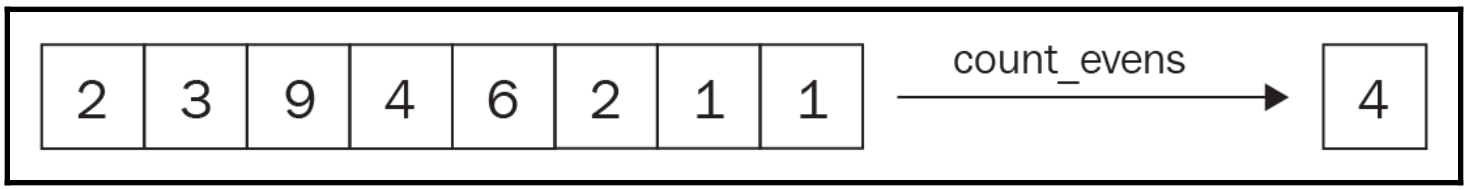
\includegraphics[width=0.6\textwidth]{content/Section-2/Chapter-7/2}
\end{center}

解决了vector的问题之后,我们应该通过将解应用到所有的向量,来继续解决最初的问题。transform()函数本质上完成了我们所需要的工作:它接受一个可以应用于单个值的函数,并对其进行转换,以处理一个集合。下面的图像说明了如何使用它来实现一个函数(count\underline{ }all\underline{ }evens),该函数可以处理来自一次只处理一个项的函数(count\underline{ }evens)的项的集合: \par

\begin{center}
	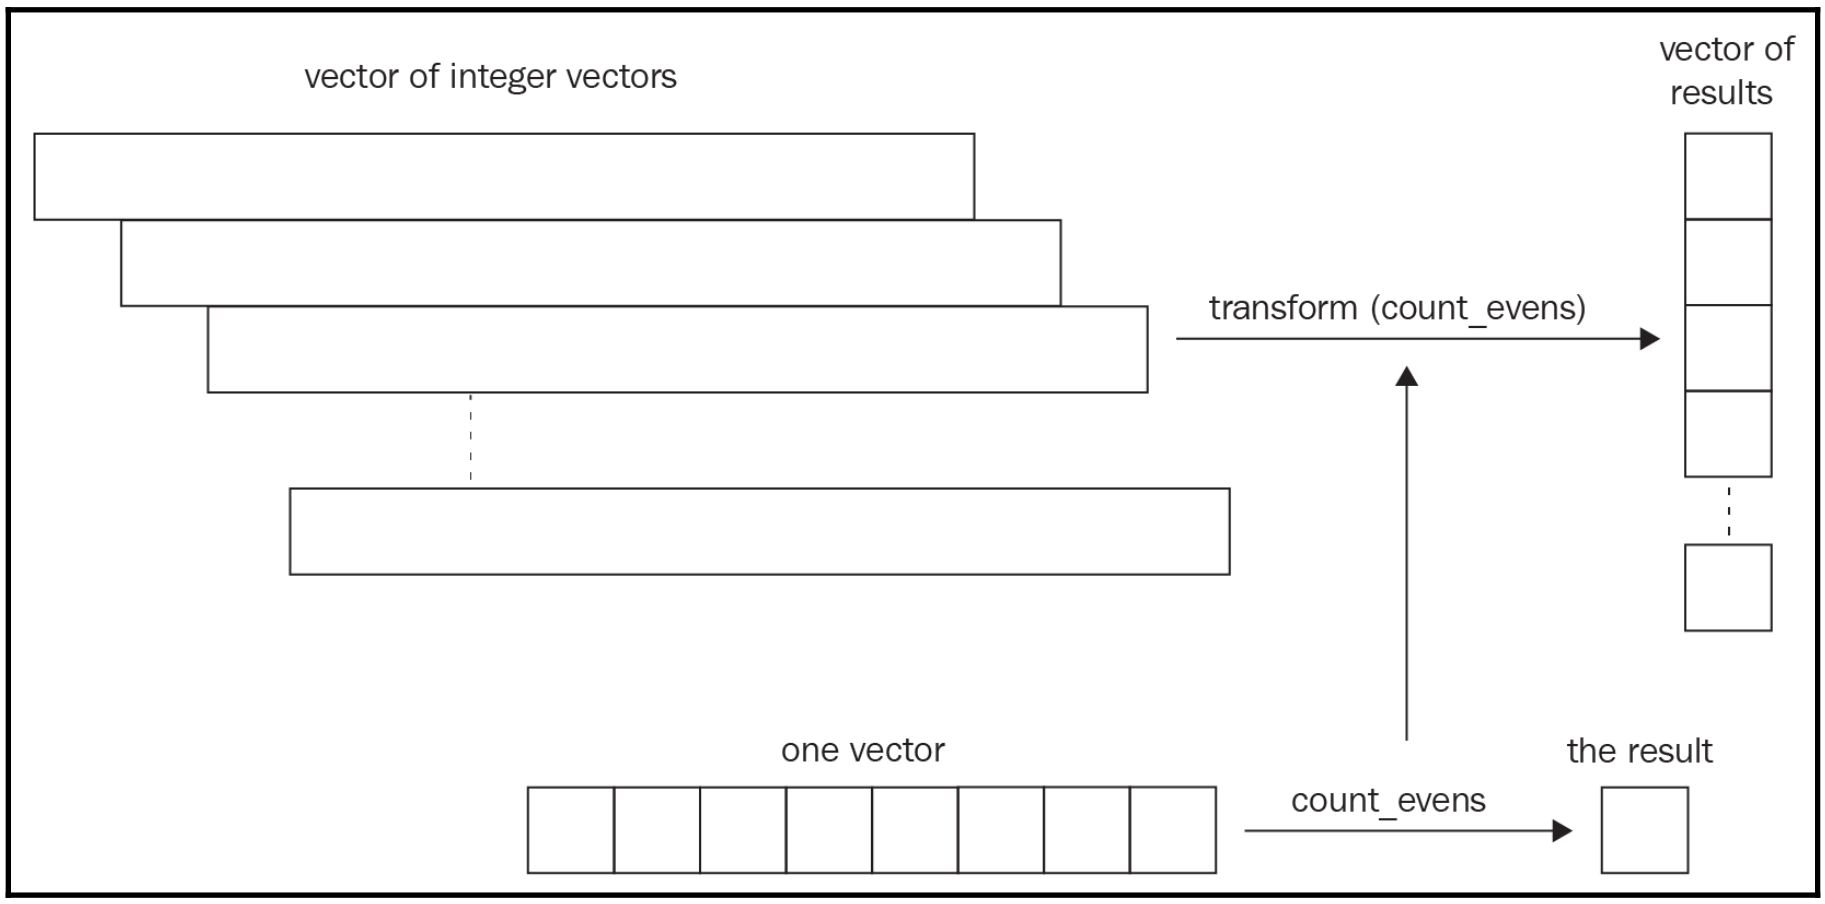
\includegraphics[width=0.6\textwidth]{content/Section-2/Chapter-7/3}
\end{center}

函数式编程的核心是,将较大的问题分解为较小的独立任务。每个函数都专门用于完成一个足够简单的任务,而没有意识到原来的问题。然后将函数组合在一起,从原始的初始输入生成一组已处理的结果。 \par
count\underline{ }all\underline{ }evens()函数的最终版本利用了range。让我们来看看range是什么,以及如何使用它。在后面的例子中,我们还会用到它。 \par

\noindent\textbf{}\ \par
\textbf{使用range} \ \par
range与view绑定,我们将在本节中对它们进行研究。它们为我们提供了一种组合和处理对象集合的通用方法。我们经常使用迭代器来遍历容器并处理其元素,迭代器允许我们对算法和容器进行解耦。 \par
例如,我们对vector应用了count\underline{ }if(),但是count\underline{ }if()不知道它会应用于哪种容器。看看以下count\underline{ }if()的声明: \par

\begin{lstlisting}[caption={}]
template <typename InputIterator, typename UnaryPredicate>
constexpr typename iterator_traits<InputIterator>::difference_type
count_if(InputIterator first, InputIterator last, UnaryPredicate p);
\end{lstlisting}

除了C++特有的详细声明之外,count\underline{ }if()不接受容器作为参数。相反,它使用迭代器操作——特别是输入迭代器。 \par

\hspace*{\fill} \\ %插入空行

\includegraphics[width=0.05\textwidth]{images/warn}
输入迭代器支持使用++操作符进行迭代,并支持使用*操作符访问每个元素。还可以使用==和!=关系来比较输入迭代器。 \par
\noindent\textbf{}\ \par

算法遍历容器而不知道容器的确切类型。可以对任何有开始和结束的实体使用count\underline{ }if(),如下所示: \par

\begin{lstlisting}[caption={}]
#include <array>
#include <iostream>
#include <algorithm>
int main()
{
	std::array<int, 4> arr{1, 2, 3, 4};
	auto res = std::count_if(arr.cbegin(), arr.cend(),
		[](int x){ return x == 3; });
	std::cout << "There are " << res << " number of elements equal to 3";
}
\end{lstlisting}

通常,我们对一个集合应用一个算法,并将该算法的结果存储为另一个集合,之后我们以同样的方式将该集合应用于更多算法。使用std::transform()将结果放入另一个容器中。例如,下面的代码定义了一个乘积向量: \par

\begin{lstlisting}[caption={}]
// consider the Product is already declared and has a "name", "price", and
"weight"
// also consider the get_products() is defined
// and returns a vector of Product instances
using ProductList = std::vector<std::shared_ptr<Product>>;
ProductList vec{get_products()};
\end{lstlisting}

假设项目是由不同的程序员团队开发的,他们选择保留产品的名称为任意数字,例如:1代表苹果,2代表桃子,以此类推。这意味着vec将包含Product实例,每个实例在其名称字段中都有一个数字字符(而名称的类型是std::string——这就是为什么我们将数字作为字符而不是其整数值)。现在,我们的任务是将产品名称从数字转换为完整字符串(apple、peach等)。我们可以使用std::transform: \par

\begin{lstlisting}[caption={}]
ProductList full_named_products; // type alias has been defined above
using ProductPtr = std::shared_ptr<Product>;
std::transform(vec.cbegin(), vec.cend(),
	std::back_inserter(full_named_products),
	[](ProductPtr p){ /* modify the name and return */ });
\end{lstlisting}

运行上述代码后,full\underline{ }named\underline{ }products将包含具有产品名的Product。为了过滤掉所有的apple并将它们复制到apple向量中,我们需要使用std::copy\underline{ }if: \par

\begin{lstlisting}[caption={}]
ProductList apples;
std::copy_if(full_named_products.cbegin(), full_named_products.cend(),
	std::back_inserter(apples),
	[](ProductPtr p){ return p->name() == "apple"; });
\end{lstlisting}

代码示例的最大缺点是在引入range之前,缺乏良好的组合。range为我们提供了一种处理容器元素和组合算法的优雅方式。 \par
简单地说,range是一个可遍历的实体,一个range有一个begin()和一个end(),这与目前为止使用的容器非常相似。这些条件下,每个STL容器都可以视为一个range。STL算法重新定义为接受范围作为直接参数,它们允许将一个结果从一个算法直接传递给另一个算法,而不是将中间结果存储在局部变量中。例如,可以在前面在begin()和end()中使用的std::transform,如果使用range,则具有以下形式(以下代码是伪代码)。通过使用range,可以按照以下方式重写前面的例子: \par

\begin{lstlisting}[caption={}]
ProductList apples = filter(
	transform(vec, [](ProductPtr p){/* normalize the name */}),
	[](ProductPtr p){return p->name() == "apple";}
);
\end{lstlisting}

不要忘记包含<ranges>头文件。transform将返回一个包含名称的Product指针的range,也就是将数值替换为字符串值。然后,filter函数将获取结果并返回名称为apple的产品range。 \par

\hspace*{\fill} \\ %插入空行

\includegraphics[width=0.05\textwidth]{images/warn}
注意,我们通过省略简化了这些代码示例
在filter和transform函数前面的std::ranges::views。相应地,使用它们作为std::ranges::views::filter和std::ranges::views::transform。 \par
\noindent\textbf{}\ \par

最后,我们在本章开头的示例中使用了重载操作符|,它允许我们在一起调用管道范围。这样,我们可以组合算法来产生最终结果,如下所示: \par

\begin{lstlisting}[caption={}]
ProductList apples = vec | transform([](ProductPtr p){/* normalize the name
	*/})
| filter([](ProductPtr p){return p->name() ==
	"apple";});
\end{lstlisting}

我们使用管道代替嵌套的函数调用。这一开始可能会令人困惑,因为我们使用|操作符作为位或。当你看到它被应用到一个集合时,它指的是管道范围。 \par

\hspace*{\fill} \\ %插入空行

\includegraphics[width=0.05\textwidth]{images/tip}
|操作符的灵感来自于Unix shell管道操作符。在Unix中,我们可以通过管道将多个进程的结果连接在一起,例如:\texttt{ls -l | grep cpp | less}将在ls命令的结果中找到cpp,并使用less程序一次显示一个屏幕的最终结果。 \par
\noindent\textbf{}\ \par

range是集合之上的抽象,这并不意味着它是一个集合。这就是为什么前面的例子没有任何开销——它只是在一个函数之间传递一个range,这个range只是提供一个集合的开始和结束。此外,还允许我们访问底层的集合元素。 \par

\begin{center}
	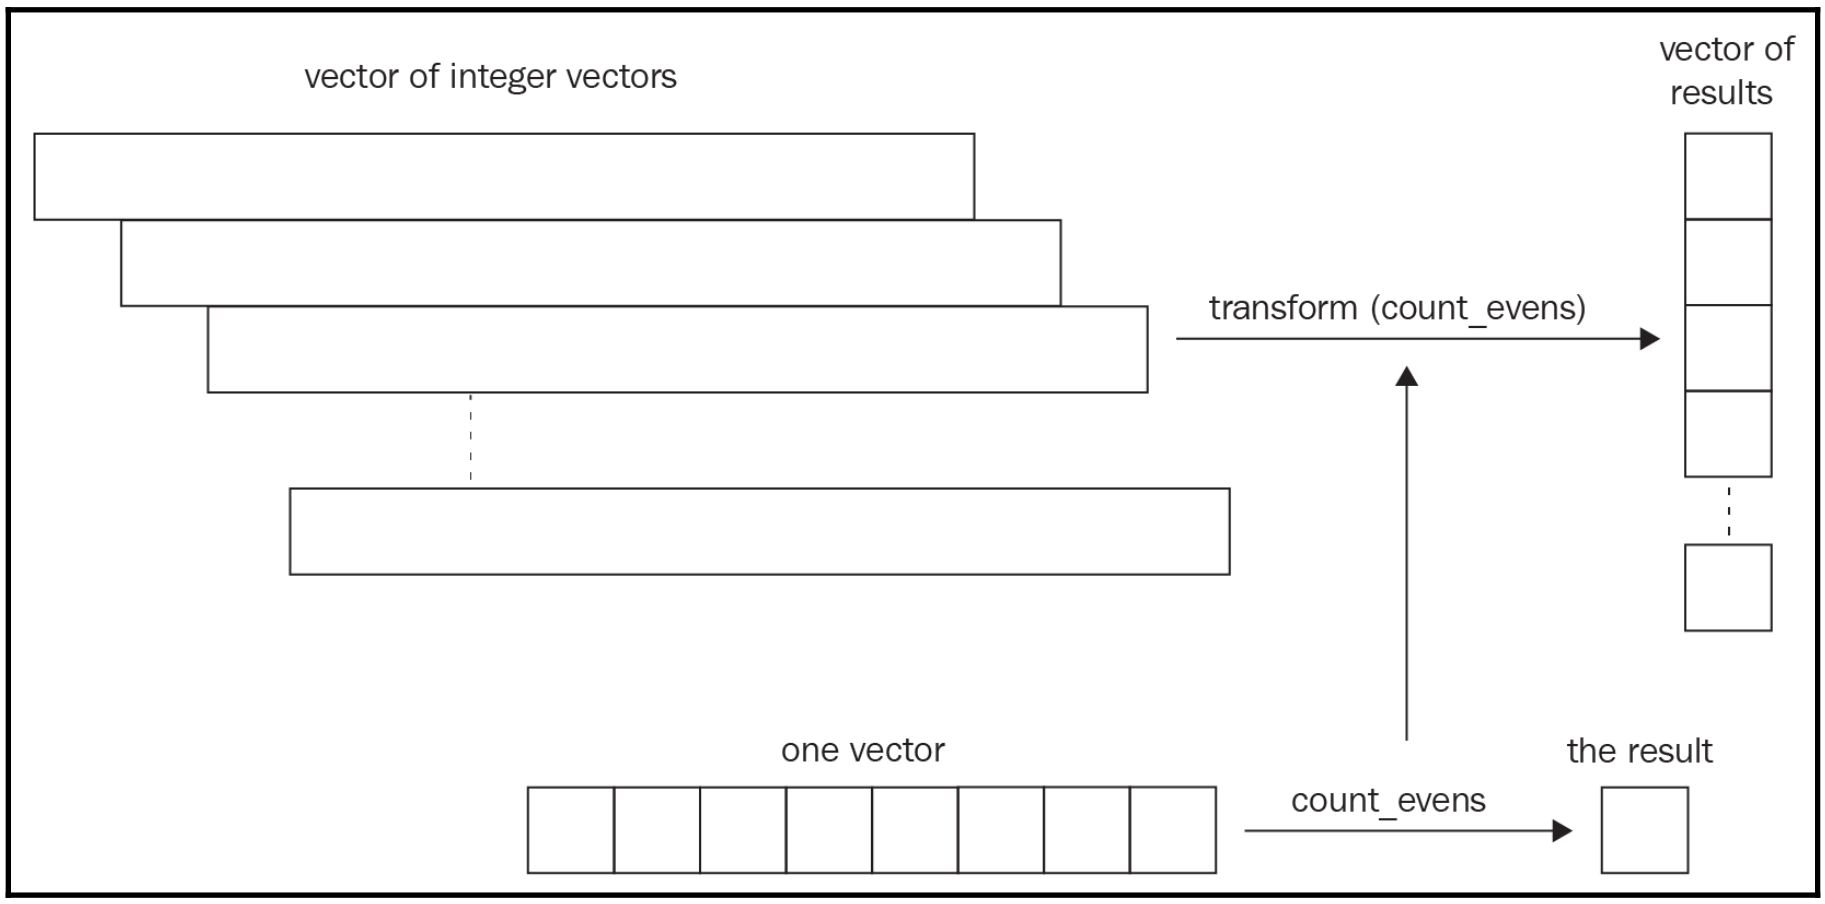
\includegraphics[width=0.6\textwidth]{content/Section-2/Chapter-7/3}
\end{center}

该函数(transform或filter)返回一个范围结构,而不是一个集合。range的begin()迭代器将指向源集合中满足谓词的元素。range的迭代器是一个代理对象:它与常规迭代器的不同之处在于,指向一个满足给定谓词的元素。我们有时将它们称为智能迭代器,因为每次向前移动它(例如,通过递增),都会找到集合中满足谓词的下一个元素。更有趣的是,迭代器的“智能”取决于我们应用于集合的函数类型。例如,filter()函数返回一个范围,该range的自增操作符具有智能迭代器。这主要是因为过滤器的结果可能比原始集合包含更少的元素。另一方面,Transform并不返回元素数量较少的结果——它只是转换元素。这意味着transform返回的range对于自增/自减操作具有相同的功能,但元素访问将有所不同。对于每次访问,range的智能迭代器将从原始集合返回转换后的元素。换句话说,只是为迭代器实现了*操作符,参考下面的代码片段: \par

\begin{lstlisting}[caption={}]
auto operator*()
{
	return predicate(*current_position);
}
\end{lstlisting}

这样,我们就创建了集合的新视图,同样适用于filter和其他函数。更有趣的是,区间视图利用了惰性求值。对于我们前面的示例,即使我们有两个range转换,结果也是通过在一次传递中求值产生的。\par
在transform和filter的示例中,每个函数都定义了一个视图,但不修改或求值。当我们将结果赋值给结果集合时,通过访问每个元素来从视图构造vector。这个vector才是求值的地方。 \par
就是这么简单——range为我们提供了带有惰性求值的函数组合。现在,我们简要地介绍了函数式编程中使用的工具集。接下来,让我们来看看这个范例的优点。 \par

\noindent\textbf{}\ \par
\textbf{为什么使用函数式编程?} \ \par
首先,函数式编程简化了代码。与命令式对应的代码相比,该代码要短得多。它提供了简单但极富表现力的工具。代码越少,bug就越少。 \par
函数不会改变任何东西,这使得并行化更加容易。这是并发程序的主要关注点之一,因为并发任务需要在它们之间共享可变数据。大多数情况下,必须使用互斥对象等显式地同步线程。函数式编程将我们从显式的同步中解放出来,我们可以在多个线程上运行代码而无需进行调整。第8章中,我们将详细讨论数据竞争。 \par
函数式编程认为所有的功能都是纯粹的,是不会改变程序状态的函数。它们只是接受输入,以用户定义的方式对其进行转换,然后提供输出。纯函数对于相同的输入生成相同的结果,而不受调用次数的影响。当我们谈到函数式编程时,在默认情况下,我们应该考虑所有纯函数。 \par
下面的函数接受double作为输入,并返回square: \par

\begin{lstlisting}[caption={}]
double square(double num) { return num * num; }
\end{lstlisting}

\hspace*{\fill} \\ %插入空行

\includegraphics[width=0.05\textwidth]{images/tip}
有些编译器,如GCC,提供帮助编译器优化代码的属性。例如,[[gnu::pure]]属性告诉编译器这个函数可以被认为是一个纯函数。这将使编译器确信函数不访问任何全局变量,并且函数的结果完全依赖于它的输入。 \par
\noindent\textbf{}\ \par

许多情况下,常规函数可以带来更快的解决方案。然而,为了适应这种模式,应该强迫自己从功能的角度思考。下面的程序声明了一个vector,并计算其元素的平方根: \par

\begin{lstlisting}[caption={}]
void calc_square_roots(std::vector<double>& vec)
{
	for (auto& elem : vec) {
		elem = std::sqrt(elem);
	}
}

int main()
{
	std::vector<double> vec{1.1, 2.2, 4.3, 5.6, 2.4};
	calc_square_roots(vec);
}
\end{lstlisting}

这里,我们通过引用传递向量。如果我们在函数中改变它,我们就改变了原始集合。这显然不是一个纯函数因为它改变了输入向量。而函数式编程将在新的vector中返回计算后的值,而不影响输入: \par

\begin{lstlisting}[caption={}]
std::vector<double> pure_calc_square_roots(const std::vector<double>& vec)
{
	std::vector<double> new_vector;
	for (const auto& elem : vec) {
		new_vector.push_back(std::sqrt(elem));
	}
	return new_vector;
}
\end{lstlisting}

功能性思维的一个更好的例子是,解决一个较小的问题并将其应用到集合中。本例中,较小的问题是计算单个数字的平方根,这个数字已经实现为std::sqrt。\\将它应用到集合是通过std::ranges::views::transform完成的,如下所示: \par

\begin{lstlisting}[caption={}]
#include <ranges>
#include <vector>

int main()
{
	std::vector<double> vec{1.1, 2.2, 4.3, 5.6, 2.4};
	auto result = vec | std::ranges::views::transform(std::sqrt);
}
\end{lstlisting}

我们使用range,可以避免存储中间对象。前面的例子中,我们直接对向量应用了transform。transform返回一个view,但不是由源向量的已转换元素组成的完整集合,而是在构造结果向量时生成元素的实际转换副本。另外,注意std::sqrt是一个纯函数。 \par
我们在本章开头解决的例子,为函数式编程提供了必要的视角。为了更好地理解这个范式,我们应该熟悉它的原理。下一节中,我们将深入研究函数式编程的原理,以便更好地了解如何,以及何时使用。 \par

\noindent\textbf{}\ \par
\textbf{函数式编程原理} \ \par
尽管函数范式已经很老了(它诞生于20世纪50年代),但它并没有席卷编程界。目前占主导地位的大多数范式包括命令式语言和面向对象语言。正如我们在本书和其他许多书中多次提到的,C++是一种多范式语言。这就是学习C++的好处:我们可以调整它以适应几乎所有的环境。掌握范式并不是一件容易的事。必须感受它并应用它,直到你最终开始从范例的角度思考。之后,将在几秒钟内看到常规任务的解决方案。 \par
如果还记得第一次学习面向对象编程是什么时候,那么可能还记得在能够释放OOP的真正潜力之前,那些有些难懂的原则,函数式编程也是如此。本节中,我们将讨论函数式编程的基本概念,这些概念将成为进一步开发的基础。可以应用(或者已经这样做了)其中的一些概念,而无需实际使用功能范例。然而,请努力理解并应用下面的每一条原则。 \par

\noindent\textbf{}\ \par
\textbf{纯函数} \ \par
如果一个函数对其他变量的状态没有影响,那么它就是纯函数。与非纯函数相比,纯函数的性能较差,因为它们避免了由于状态修改而在代码中出现的大多数bug。程序使用数据,因此使用状态修改功能,为最终用户带来一些预期的结果。 \par
在面向对象编程中,我们将程序分解为对象,每一个对象都有一系列特殊的特性。OOP中对象的基本特性之一是它的状态。通过向对象发送消息(换句话说,调用其方法)来修改对象的状态,在OOP中是至关重要的。通常,成员函数调用会导致对象状态的修改。函数式编程中,我们将代码组织成纯函数的集合,每个函数都有自己的目的,并且独立于其他函数。 \par
我们看一个简单的例子,只是为了使这个概念更清楚。假设我们在一个程序中处理User对象,每个User对象都包含与User相关的信息。User类在下面的代码块中声明为一个结构体: \par

\begin{lstlisting}[caption={}]
struct User
{
	int age;
	string name;
	string phone_number;
	string email;
};
\end{lstlisting}

需要每年更新用户的年龄,假设我们有一个每年为每个User对象调用一次的函数。下面的函数接受一个User对象作为输入,并将其年龄增加1: \par

\begin{lstlisting}[caption={}]
void update_age(User& u)
{
	u.age = u.age + 1;
}
\end{lstlisting}

update\underline{ }age()函数通过引用接受输入,并更新原始对象。但在函数式编程中却不是这样。下面的纯函数不是通过引用来获取原始对象,并改变其值,而是返回一个具有相同属性的User对象,只是更新了age属性: \par

\begin{lstlisting}[caption={}]
User pure_update_age(const User& u) // cannot modify the input argument
{
	User tmp{u};
	tmp.age = tmp.age + 1;
	return tmp;
}
\end{lstlisting}

尽管与update\underline{ }age()相比,看起来效率较低,但这种方法的优点是使操作变得非常清晰(这在调试代码时非常有用),可以保证pure\underline{ }update\underline{ }age()不会修改原始对象。我们可以修改前面的代码,使它按值接受对象。这样,我们将跳过tmp对象的创建,因为实参本身表示为一个副本: \par

\begin{lstlisting}[caption={}]
User pure_update_age(User u) // u is the copy of the passed object
{
	u.age = u.age + 1;
	return u;
}
\end{lstlisting}

如果用相同的参数多次调用纯函数,则每次都必须返回相同的结果。下面的代码演示了pure\underline{ }update\underline{ }age()函数在给定相同的输入时,返回相同的值: \par

\begin{lstlisting}[caption={}]
User john{.age{21}, .name{"John"}};

auto updated{pure_update_age(john)};
std::cout << updated.age; // prints 22

updated = pure_update_age(john);
std::cout << updated.age; // prints 22
\end{lstlisting}

对于函数来说,每次为相同的输入数据调用它时,都可以以相同的方式运行。这意味着可以通过将应用程序分解成更小的函数,来设计应用程序的逻辑,每个函数都有明确的目的。然而,就额外的临时对象而言,纯函数有开销。常规的设计包括有一个集中存储程序状态的存储,由纯函数间接更新。每次使用纯函数后,该函数将修改后的对象作为新对象返回,必要时可以存储该对象。可以将其视为调整代码,以忽略传递的对象。 \par

\noindent\textbf{}\ \par
\textbf{高阶函数} \ \par
函数式编程中,函数是一等对象。我们应该把函数当作对象,而不是一组指令。这对我们有什么区别?此时,要将一个函数视为对象,体现的是将它传递给其他函数的能力。接受其他函数作为参数的函数称为高阶函数。 \par
C++开发者将一个函数传递给另一个函数并不少见。下面是一些经典的方法: \par

\begin{lstlisting}[caption={}]
typedef void (*PF)(int);
void foo(int arg)
{
	// do something with arg
}

int bar(int arg, PF f)
{
	f(arg);
	return arg;
}

bar(42, foo);
\end{lstlisting}

代码中,声明了一个指向函数的指针。PF表示函数的类型,接受一个整型参数,不返回任何值。示例是将指针函数作为参数,传递给其他函数的一种方法。我们把函数看作为一个对象,这需要我们对对象更深的理解。 \par
前面的章节中,我们将对象定义为具有状态的东西。如果将函数视为对象,我们也应该能够在需要时以某种方式改变其状态。对于函数指针,情况并非如此。下面是传递一个函数给另一个函数的更好方法: \par

\begin{lstlisting}[caption={}]
class Function
{
public:
	void modify_state(int a) {
		state_ = a;
	}
	int get_state() {
		return state_;
	}
	void operator()() {
		// do something that a function would do
	}
private:
	int state_;
};
void foo(Function f)
{
	f();
	// some other useful code
}
\end{lstlisting}

声明了一个具有重载函数操作符的类。每当重载类的操作符时,就使其可调用。因此,具有重载函数操作符的类对象可以视为函数(也称为函子)。这在某种程度上更像是一个技巧,因为我们没有把函数变成对象,而是把对象变成了可调用的函数。然而,这让我们能够实现我们所寻找的:一个具有状态的函数。下面的客户端代码演示了函数对象有一个状态: \par

\begin{lstlisting}[caption={}]
void foo(Function f)
{
	f();
	f.modify_state(11);
	cout << f.get_state(); // get the state
	f(); // call the "function"
}
\end{lstlisting}

通过这样做,我们可以跟踪函数被调用了多少次。下面是一个跟踪调用数量的简单示例: \par

\begin{lstlisting}[caption={}]
class Function
{
public:
	void operator()() {
		// some useful stuff
		++called_;
	}
private:
	int called_ = 0;
};
\end{lstlisting}

最后,在<functional>头文件中定义的std::function演示了另一种定义高阶函数的方法: \par

\begin{lstlisting}[caption={}]
#include <functional>

void print_it(int a) {
	cout << a;
}
std::function<void(int)> function_object = print_it;
\end{lstlisting}

当调用function\underline{ }object时(使用()),它将调用委托给print\underline{ }it函数。function封装了函数,并允许将其作为对象使用(并将其传递给其他函数)。 \par
例子中以其他函数作为参数的函数,都是高阶函数的例子。返回函数的函数也称为高阶函数。总而言之,高阶函数是接受或返回另一个或多个函数的函数。看看下面的例子: \par

\begin{lstlisting}[caption={}]
#include <functional>
#include <iostream>

std::function<int (int, int)> get_multiplier()
{
	return [](int a, int b) { return a * b; };
}

int main()
{
	auto multiply = get_multiplier();
	std::cout << multiply(3, 5) << std::endl; // outputs 15
}
\end{lstlisting}

get\underline{ }multiplier()返回一个用std::function包装的lambda函数。然后调用,就像调用一个常规函数一样。get\underline{ }multiplier()函数是一个高阶函数。我们可以使用高阶函数实现套用。函数式编程中,套用就是将一个函数带几个参数放入几个函数中,每个函数带一个参数,例如:将multiply(3,5)变为multiply(3)(5)。我们可以这样做: \par

\begin{lstlisting}[caption={}]
std::function<int(int)> multiply(int a)
{
	return [a](int b) { return a * b; };
}

int main()
{
	std::cout << multiply(3)(5) << std::endl;
}
\end{lstlisting}

multiply()只接受一个参数,返回的函数也只有一个参数。请注意lambda捕获:它捕获a的值,以便在它的体中将其乘以b。 \par

\hspace*{\fill} \\ %插入空行

\includegraphics[width=0.05\textwidth]{images/warn}
Curry指的是逻辑学家Haskell Curry。Haskell、Brook和Curry编程语言也以他的名字命名。 \par
\noindent\textbf{}\ \par

套用的一个最有用的特性是,可以将抽象函数组合在一起。我们可以创建multiply()的特化版本,并将其传递给其他函数,或者在任何合适的地方使用。这可以在下面的代码中看到: \par

\begin{lstlisting}[caption={}]
auto multiplyBy22 = multiply(22);
auto fiveTimes = multiply(5);

std::cout << multiplyBy22(10); // outputs 220
std::cout << fiveTimes(4); // outputs 20
\end{lstlisting}

使用STL时,一定使用了高阶函数。许多STL算法使用谓词来过滤或处理对象集合,例如:std::find\underline{ }if函数查找满足传递的谓词对象的元素,如下面的示例所示: \par

\begin{lstlisting}[caption={}]
std::vector<int> elems{1, 2, 3, 4, 5, 6};
std::find_if(elems.begin(), elems.end(), [](int el) {return el % 3 == 0;});
\end{lstlisting}

std::find\underline{ }if将lambda作为其谓词,并对vector中的所有元素使用它。满足条件的元素将作为请求的元素返回。 \par
另一个高阶函数的例子是std::transform,我们在本章开始时介绍过(不要与ranges::view::transform混淆)。让我们用它把一个字符串转换成大写字母: \par

\begin{lstlisting}[caption={}]
std::string str = "lowercase";
std::transform(str.begin(), str.end(), str.begin(),
	[](unsigned char c) { return std::toupper(c); });
std::cout << str; // "LOWERCASE"
\end{lstlisting}

第三个形参是容器的开头,也是std::transform函数插入其当前结果的地方。 \par

\noindent\textbf{}\ \par
\textbf{折叠表达式} \ \par
折叠(或简化)是将一组值组合在一起以生成较少结果的过程。大多数时候,我们谈论的是单一的结果。折叠抽象了递归的结构上迭代的过程。例如,就元素访问而言,list或vector具有递归性质。虽然vector的递归性质具有争议,但我们将其视为递归,因为它允许我们通过重复递增索引来访问其元素。为了处理这样的结构,我们通常会跟踪每一步的结果,然后处理下一个项目,以便稍后与前一个结果结合。根据我们处理集合元素的方向,折叠称为左折叠或右折叠。 \par
例如,std::accumulate函数(另一个高阶函数的例子)是折叠功能的完美例子,因为它组合了集合中的值。看看下面这个简单的例子: \par

\begin{lstlisting}[caption={}]
std::vector<double> elems{1.1, 2.2, 3.3, 4.4, 5.5};
auto sum = std::accumulate(elems.begin(), elems.end(), 0);
\end{lstlisting}

函数的最后一个参数是累加器。这个初始值应该用作集合第一个元素的前一个值。上面的代码计算vector元素的和。这是std::accumulate函数的默认行为。正如我们前面提到的,它是一个高阶函数,这意味着函数可以作为它的参数传递。然后对每个元素调用这个函数,以产生所需的结果,例如:找到前面声明的elems向量的乘积: \par

\begin{lstlisting}[caption={}]
auto product = std::accumulate(elems.begin(), elems.end(), 1, [](int prev, int cur) { return prev * cur; });
\end{lstlisting}

需要一个有两个参数的函数,第一个参数是计算的前一个值,第二个参数是当前值。操作的结果将是下一个步骤的前一个值。代码可以用STL中的操作,以简洁的方式重写: \par

\begin{lstlisting}[caption={}]
auto product = std::accumulate(elems.begin(), elems.end(), 1, std::multiplies<int>());
\end{lstlisting}

std::accumulate函数的更好替代是std::reduce函数。reduce()类似于accumulate(),不同的是它不保持操作的顺序,它不必按顺序处理集合元素。可以将执行策略传递给std::reduce函数,并更改其行为,比如:并行处理元素。下面是如何使用并行执行策略,将reduce函数应用于前面例子中的elems: \par

\begin{lstlisting}[caption={}]
std::reduce(std::execution::par, elems.begin(), elems.end(), 1, std::multiplies<int>());
\end{lstlisting}

虽然std::reduce看起来比std::accumulate快,但是在使用非交换二元操作时应该小心。 \par
折叠和递归密不可分。递归函数也通过将问题分解成更小的任务,逐个解决来解决整个问题。 \par

\noindent\textbf{}\ \par
\textbf{深入地研究递归} \ \par
第2章中讨论了递归函数的主要特性。来看看以下递归计算一个数字的阶乘的简单例子: \par

\begin{lstlisting}[caption={}]
int factorial(int n)
{
	if (n <= 1) return 1;
	return n * factorial(n - 1);
}
\end{lstlisting}

与迭代函数相比,递归函数提供了优雅的解决方案。但是,应该谨慎地决定是否使用递归。递归函数最常见的问题之一是堆栈溢出。 \par

\noindent\textbf{}\ \par
\textbf{头递归} \ \par
头递归是我们熟悉的常规递归方式。前面的例子中,factorial函数的行为就是一个头递归函数,它在处理当前步骤的结果之前进行递归调用。看一下阶乘函数的下面一行: \par

\begin{lstlisting}[caption={}]
...
return n * factorial(n - 1);
...
\end{lstlisting}

为了找到并返回乘积的结果,调用factorial函数,并带有一个简化的参数,即(n-1)。这意味着乘积(*操作符)在某种程度上处于暂停状态,正在等待它的第二个参数通过阶乘(n-1)返回。堆栈的增长与递归调用函数的次数一致,让我们试着比较一下递归阶乘的实现和下面的迭代方法: \par

\begin{lstlisting}[caption={}]
int factorial(int n)
{
	int result = 1;
	for (int ix = n; ix > 1; --ix) {
		result *= ix;
	}
	return result;
}
\end{lstlisting}

这里的主要区别是,在每一步都将product的结果存储在同一个变量(名为result)中。让我们尝试分解阶乘函数的递归实现。 \par
很明显,每个函数调用都会占用堆栈上指定的空间。每个步骤的每个结果都应该存储在堆栈的某个地方。虽然我们知道它应该是同一个变量,但递归函数并不关心,它会为变量分配空间。常规递归函数要求我们找到一种解决方案,即知道每个递归调用的结果应该存储在相同的地方。 \par

\noindent\textbf{}\ \par
\textbf{尾递归} \ \par
尾递归是解决递归函数中存在多个不必要变量问题的方法。尾递归函数的基本思想是在递归调用之前进行实际处理。下面是我们如何将阶乘函数转换为尾递归函数: \par

\begin{lstlisting}[caption={}]
int tail_factorial(int n, int result)
{
	if (n <= 1) return result;
	return tail_factorial(n - 1, n * result);
}
\end{lstlisting}

注意函数的新参数。仔细阅读前面的代码,我们可以了解正在发生的尾递归的基本概念:处理在递归调用之前完成在tail\underline{ }factorial函数再次调用之前,计算当前的结果(n * result)并传递给它。 \par
虽然这种想法看起来并不吸引人,但如果编译器支持尾部调用优化(TCO),它就会非常高效。TCO基本上涉及到阶乘函数(尾部)的第二个参数可以在每次递归调用时存储在相同的位置。这允许堆栈保持相同的大小,独立于递归调用的数量。 \par
说到编译器优化,我们不能忽略模板元编程。我们在这里与编译器优化一起提到它,可以将元编程视为对程序的最大优化。编译时进行计算总是比在运行时进行计算更好。 \par

\noindent\textbf{}\ \par
\textbf{C++中(函数式)的元编程} \ \par
元编程可以看作是另一种编程范式,是一种完全不同的编码方法,因为不是在处理常规的编程过程。所谓常规过程,我们指的是程序在其生命周期中所经历的三个阶段:编码、编译和运行。很明显,一个程序在执行时做了它应该做的事情,可执行文件由编译器通过编译和链接生成。另一方面,元编程是代码编译期间执行代码的地方。如果你是第一次面对它,这听起来可能很神奇。如果程序还不存在,我们怎么执行代码?回顾第4章中关于模板的内容,我们知道编译器处理模板需要多次传递。第一次传递中,编译器定义模板类或函数中使用的必要类型和形参。接下来,编译器开始用我们熟悉的方式编译,它生成一些代码,这些代码将被链接器链接,以生成最终的可执行文件。 \par
由于元编程是在代码编译过程中发生,我们应该知道使用了哪些语言概念和结构。任何可以在编译时计算的东西都可以用作元编程构造,比如:模板。 \par
下面是用C++进行元编程的经典例子: \par

\begin{lstlisting}[caption={}]
template <int N>
struct MetaFactorial
{
	enum {
		value = N * MetaFactorial<N - 1>::value
	};
};

template <>
struct MetaFactorial<0>
{
	enum {
		value = 1
	};
};

int main() {
	std::cout << MetaFactorial<5>::value; // outputs 120
	std::cout << MetaFactorial<6>::value; // outputs 720
}
\end{lstlisting}

我们在上一节用不到5行代码编写了阶乘,为什么要为阶乘写这么多代码呢?原因在于它的效率。虽然编译代码需要花费更多的时间,但与普通的阶乘函数(递归或迭代实现)相比,是高效的。这种效率背后的原因是,实际的阶乘计算是在编译时进行的,当可执行文件运行时,结果已经可以使用了。我们只是在运行程序时使用了计算值,运行时不进行计算。如果是第一次看到这段代码,下面的解释会让您爱上元编程。 \par
让我们详细分解和分析前面的代码。首先,元阶乘模板是用带有value属性的单个enum声明的。选择此enum仅仅是因为它的属性是在编译时计算的。因此,当我们访问MetaFactorial的value属性时,它已经在编译时计算(评估)了。看看枚举的实际值。它从相同的元阶乘类中建立递归依赖: \par

\begin{lstlisting}[caption={}]
template <int N>
struct MetaFactorial
{
	enum {
		value = N * MetaFactorial<N - 1>::value
	};
};
\end{lstlisting}

聪明的你可能已经注意到了这个技巧。MetaFactorial<N - 1>和MetaFactorial<N>不是同一个结构。尽管具有相同的名称,但是具有不同类型或值的每个模板都将作为单独的新类型生成。所以,我们调用类似这样的东西: \par

\begin{lstlisting}[caption={}]
std::cout << MetaFactorial<3>::value;
\end{lstlisting}

编译器会为每个值生成三个不同的结构体(下面是一些表示我们应该如何描绘编译器工作的伪代码): \par

\begin{lstlisting}[caption={}]
struct MetaFactorial<3>
{
	enum {
		value = 3 * MetaFactorial<2>::value
	};
};

struct MetaFactorial<2>
{
	enum {
		value = 2 * MetaFactorial<1>::value;
	};
};

struct MetaFactorial<1>
{
	enum {
		value = 1 * MetaFactorial<0>::value;
	};
};
\end{lstlisting}

下一段代码中,编译器将生成的每个结构体的值替换为各自的数值,如下面的伪代码所示: \par

\begin{lstlisting}[caption={}]
struct MetaFactorial<3>
{
	enum {
		value = 3 * 2
	};
};

struct MetaFactorial<2>
{
	enum {
		value = 2 * 1
	};
};

struct MetaFactorial<1>
{
	enum {
		value = 1 * 1
	};
};
\end{lstlisting}

然后,编译器删除未使用的生成的结构,只留下MetaFactorial<3>,如同MetaFactorial<3>::value一样。这也可以进行优化。这样做,我们可以得到如下结果: \par

\begin{lstlisting}[caption={}]
std::cout << 6;
\end{lstlisting}

将这一行与前面的行进行比较: \par

\begin{lstlisting}[caption={}]
std::cout << MetaFactorial<3>::value;
\end{lstlisting}

这就是元编程的美妙之处——在编译时完成,不会留下任何痕迹,就像忍者一样。与常规解决方案相比,编译需要更长的时间,但程序的执行速度是最快的。我们建议读者们尝试实现其他代价昂贵的计算的元版本,例如:计算第n个斐波那契数。这并不像为运行时编写代码那么简单,但是现在读者们已经对它的强大功能有了一定的了解。\par

\noindent\textbf{}\ \par
\textbf{总结} \ \par
本章中,我们有了一个新视角。作为一种多范式语言,C++可以用作函数式编程语言。 \par
我们学习了函数式编程的主要原理,如:纯函数、高阶函数和折叠表达式。纯函数不会改变状态的函数。纯函数的优点是,避免由于状态突变而引入的bug。 \par
高阶函数是接受或返回其他函数的函数。与函数式编程不同,C++开发者在处理STL时使用高阶函数。 \par
纯函数,以及高阶函数,允许我们将整个应用程序分解成一个大的函数流水线。这个流水线中的每个函数负责接收数据并返回原始数据的新修改版本(不改变原始状态)。当这些功能组合在一起时,提供了一个协调良好的任务组。 \par
下一章中,我们将深入研究多线程编程,并讨论C++中的线程库组件。 \par

\noindent\textbf{}\ \par
\textbf{问题} \ \par
\begin{enumerate}
	\item 列出range的优点。
	\item 已知哪些函数是纯函数?
	\item 从函数式编程的角度来看,纯虚函数和纯函数有什么区别?
	\item 什么是折叠表达式?
	\item 尾递归比头递归有什么好处?
\end{enumerate}

\noindent\textbf{}\ \par
\textbf{扩展阅读} \ \par
有关本章内容的更多信息,请查看以下链接: \par

\begin{itemize}
	\item Learning C++ Functional Programming by Wisnu Anggoro:  https:/​/​www.packtpub.​com/​application-​development/​learning-​c-​functional-​programming
	\item Functional Programming in C++: How to Improve Your C++ Programs Using Functional Techniques by Ivan Cukic:  https:/​/​www.​amazon.​com/​Functional-Programming-​programs-​functional-​techniques/​dp/​1617293814/​
\end{itemize}

\newpage







